\subsection{Problem 4: Atap Seng di Siang Bolong}

\subsubsection{Identifikasi Masalah}
\begin{itemize}
\item \textbf{Kriteria 2: \textit{event time vs processing time}, \textit{watermark} dan \textit{allowed lateness}.} Deteksi harus dikelompokkan berdasarkan waktu lintasan satelit, bukan waktu tiba. Data yang terlambat harus diberi batas yang dinyatakan dan dihitung bila melewatinya (Akidau dkk., \textit{The Dataflow Model}, dan \textit{Streaming Systems}).
\item \textbf{Kriteria 4: \textit{backpressure} dan \textit{consumer lag}} saat aliran dipercepat 60$\times$. Latensi dari masuk sampai tersimpan harus terukur.
\item \textbf{Kriteria 5: \textit{stateful stream processing} dengan \textit{checkpoint} dan \textit{exactly-once processing}.} Keadaan kebakaran yang sedang dibentuk dan posisi baca harus tersimpan secara atomik agar \textit{crash} tidak menghilangkan atau menggandakan kebakaran.
\item \textbf{Kriteria 1 dan 3:} pengelompokan berantai (\textit{connected components}) dan \textit{stable identifiers} untuk kebakaran yang diperbarui, digabung, atau ditarik.
\end{itemize}

\subsubsection{Rancangan Solusi}

\begin{longtable}{|p{3.5cm}|p{11.4cm}|}
\hline
\textbf{Aspek} & \textbf{Desain}\\ \hline \endhead
Pengambilan data & \kode{GET /v1/stream} (SSE, token grup dari Secret). \textit{Reconnect} dengan \kode{?from=<offset>}. 400/401 menghentikan service. 429/503 \textit{backoff} eksponensial (menghormati \kode{Retry-After}). 45 s tanpa \textit{byte} memicu \textit{reconnect}.\\ \hline
Lanjut setelah \textit{restart} & \textit{Offset} berikutnya disimpan di PostgreSQL \textbf{dalam transaksi yang sama} dengan perubahan kebakaran.\\ \hline
Definisi kebakaran & Dedup \kode{satellite|acq\_date|acq\_time|lat|lon}. Buang \textit{confidence} rendah. Hubungkan deteksi $\le$ 1 km dan $\le$ 360 menit secara berantai. $\ge$ 2 deteksi = kebakaran. Deteksi tunggal dihitung.\\ \hline
Waktu & Seluruh logika memakai waktu akuisisi deteksi (UTC), bukan waktu tiba.\\ \hline
Keterlambatan & Deteksi yang lebih tua 2 jam dari deteksi terbaru yang pernah dilihat dihitung sebagai \textit{late} dan tidak dikelompokkan (\kode{satellite\_durable\_count\{kind="late"\}}).\\ \hline
\textit{Update}/\textit{retract} & Mengubah deteksi tersimpan dan mengelompokkan ulang hanya kebakaran terkait. Deteksi yang ditarik tetap disimpan dengan tanda.\\ \hline
ID stabil & \kode{source\_ref\_id} diawali hash kunci deteksi paling awal, lalu dibawa ke kebakaran hasil hitung ulang yang beririsan. Saat digabung, kebakaran lama mempertahankan ID dan yang lain dikirim sebagai \textit{delete}.\\ \hline
Pemetaan & WILDFIRE/SATELIT. Lokasi berupa \textit{centroid}. \kode{occurred\_at} deteksi paling awal. Provinsi terdekat (tabel statis 38 provinsi). \textit{Severity} AWAS ($\ge$ 20 deteksi atau $\ge$ 100 MW), SIAGA ($\ge$ 6 atau $\ge$ 30 MW), WASPADA. \kode{attributes}: \kode{detection\_count}, \kode{satellites}, \kode{max\_confidence}, \kode{total\_frp\_mw}, \kode{detection\_keys}.\\ \hline
Pengiriman ke Aggregator & \textit{Outbox} dalam transaksi yang sama, dipublikasikan ke \kode{hazard.ingest.SATELIT} dengan \kode{Nats-Msg-Id}. \kode{source\_version} = \textit{offset} feed sehingga keadaan terbaru selalu menang. Bila satu kebakaran punya beberapa baris \textit{outbox} yang belum terkirim, \textit{relay} hanya mengirim yang terbaru dan menandai yang lama sebagai tergantikan (\kode{satellite\_outbox\_superseded\_total}), karena Aggregator tetap hanya menyimpan versi tertinggi. Ini mencegah lonjakan \textit{update} saat mengejar \textit{backlog} membanjiri Aggregator.\\ \hline
Duplikat dari feed & Feed mengirim ulang sebagian deteksi. Kunci yang sudah pernah disimpan diabaikan dan dihitung sebagai \textit{duplicate}, sehingga salinan ulang tidak membatalkan \textit{update} yang datang kemudian dan tidak menghidupkan kembali deteksi yang sudah ditarik.\\ \hline
Pengelompokan ulang & Hanya bagian yang terdampak satu pesan: tetangga langsung deteksi baru ($\le$ 1 km, $\le$ 360 menit) beserta kebakaran tempat tetangga itu berada, atau kebakaran yang memuat deteksi yang diubah. Kebakaran tersimpan adalah komponen terhubung yang lengkap, sehingga tidak ada deteksi lain yang dapat ikut terhubung. Hasilnya sama dengan mengelompokkan ulang seluruh data, tanpa biaya yang tumbuh dengan jumlah data.\\ \hline
Event rusak & Baris lebih dari 1 MiB, JSON rusak, deteksi tidak valid, dan \textit{panic} saat memproses satu pesan disimpan di \kode{satellite\_dead\_letters} beserta \textit{byte} mentahnya. \textit{Offset} tetap maju sehingga satu event rusak tidak menghentikan aliran.\\ \hline
\end{longtable}

\subsubsection{Alasan Keputusan}
\begin{itemize}
\item \textbf{SSE + \textit{offset} vs \textit{polling} M1:} Aliran berbasis \textit{offset} monoton memberi posisi baca yang tepat untuk dilanjutkan, tanpa \textit{watermark} waktu yang bisa melewatkan atau mengulang data seperti pada \textit{polling} berbasis \kode{since}.
\item \textbf{Keadaan di PostgreSQL milik ingestor vs JetStream KV:} \textit{offset}, deteksi, kebakaran, dan \textit{outbox} perlu diperbarui atomik. Satu transaksi PostgreSQL memberikannya tanpa protokol dua fase. JetStream KV tidak dapat ikut dalam transaksi yang sama dengan tabel kebakaran, sehingga \textit{crash} di antara dua penulisan dapat membuat \textit{offset} dan keadaan tidak sinkron.
\item \textbf{Batas keterlambatan 2 jam:} batas yang lebih besar menerima lebih banyak deteksi terlambat, tetapi kebakaran baru stabil lebih lama dan lebih banyak keadaan lama yang harus dihitung ulang. Batas yang lebih kecil membuang lebih banyak data. Dua jam jauh lebih pendek dari jendela penghubung 360 menit, sehingga deteksi yang diterima masih dapat menyambung ke kebakaran yang sedang dibentuk. Pada feed latihan (181.467 event), batas ini menghitung 4.845 deteksi (2,7\%) sebagai \textit{late}. Sisanya diterima. Nilainya diukur dari waktu deteksi terbaru yang pernah dilihat (\textit{watermark} \textit{event time}), bukan dari jam dinding, karena feed berjalan pada waktu virtual 60$\times$.
\end{itemize}

\subsubsection{Batasan yang Disadari}
\begin{itemize}
\item \kode{satellite-ingestor} berjalan satu replika (\textit{Recreate}). Dua replika bersamaan akan membaca feed dua kali.
\item Pemetaan provinsi memakai jarak ke ibu kota provinsi, sehingga titik dekat perbatasan dapat dinamai provinsi tetangga.
\item Deteksi yang melewati batas keterlambatan hanya dihitung, tidak disimpan, sehingga tidak dapat dikelompokkan belakangan bila batas diubah.
\item Event satelit yang rusak tersimpan di \kode{satellite\_dead\_letters}, terpisah dari DLQ Aggregator, sehingga tidak muncul di \kode{/internal/audit/unprocessed}.
\item Uji \textit{kill-and-restart} memakai rekaman feed profil \textit{practice}. Profil ujian asisten tidak diuji.
\item Jaeger menyimpan 5\% \textit{trace} \kode{satellite-ingestor}, sehingga tidak setiap pesan dapat dilacak.
\item Pada Docker Compose, satu Aggregator menerapkan $\pm$10--20 pesan/s karena setiap pesan, termasuk versi lama yang diabaikan, memerlukan satu transaksi CockroachDB. Sebelum \textit{relay} menggabungkan versi per kebakaran, ingestor yang sedang mengejar \textit{backlog} mengirim lebih cepat dari itu dan antrean Aggregator sempat mencapai $\pm$158 ribu pesan. Latensi p50/p95/p99 pada kriteria 4 diukur di ingestor (dari baca sampai komit), bukan sampai HazardEvent tersimpan di \kode{canonical\_events}.
\end{itemize}

\subsubsection{Bukti Penyelesaian}

\begin{longtable}{|p{4.2cm}|p{10.7cm}|}
\hline
\textbf{Kriteria} & \textbf{Bukti}\\ \hline \endhead
\multicolumn{2}{|p{14.9cm}|}{Bukti kriteria 1--4, 7, dan 8 dikumpulkan oleh \kode{scripts/demo/m2/p4/p4.sh} ke \kode{evidence/p4/<run>/}. Angka di bawah diambil dari \kode{summary.txt} run \kode{20261122T073253Z} (Docker Compose) kecuali disebut lain.}\\ \hline
1. WILDFIRE & \kode{satellite-fires-top.txt} dan \kode{canonical-wildfire-top.txt}: contoh HazardEvent WILDFIRE \kode{1d7fd1e3\ldots}, AWAS, Jawa Timur, \kode{occurred\_at} 2026-12-03 03:34 UTC, 62 deteksi. Setelah antrean Aggregator habis, \kode{satellite-store} berisi 7.980 kebakaran dan \kode{canonical\_events} berisi 7.920 WILDFIRE aktif serta 18 yang dihapus. Selisih 60 adalah pesan yang masih dalam perjalanan. Sebaran \textit{severity} di \kode{satellite-store}: 7.557 AWAS, 29 WASPADA, karena total FRP dijumlahkan sepanjang umur kebakaran.\\ \hline
2. Waktu deteksi, keterlambatan & Pada feed latihan: 4.845 \textit{late}, 19.883 \textit{confidence} rendah, 9.259 duplikat dari 181.467 event. Feed \textit{live} (483.254 \textit{offset}): 13.033 \textit{late}, 53.075 \textit{confidence} rendah, 24.602 duplikat, 5.474 kunci tak dikenal, 0 tidak valid, 0 \textit{dead letter}.\\ \hline
3. \textit{Update}/\textit{retract} & \kode{stable-id-history.txt}: kebakaran \kode{fb89a3a5\ldots} mempertahankan \kode{source\_ref\_id} yang sama selama 101 versi. 30 pesan \textit{delete} (kebakaran yang tergabung atau kosong) dan 8.129 deteksi ditarik. Kasus penarikan deteksi paling awal, penggabungan, dan pemisahan diuji di \kode{internal/ingest}.\\ \hline
4. 60$\times$, p95 latensi & Pada rekaman feed latihan (uji \kode{internal/e2e}, tanpa jaringan), pemrosesan $\pm$385 event/s. Feed \textit{live} 60$\times$ (Compose): latensi dari masuk sampai tersimpan di ingestor p50 15,6 ms, p95 44,6 ms, p99 76,3 ms. Pada tiga pengukuran 60 detik, ingestor membaca 54,5--77,9 event/s, sedangkan feed bertambah 0,3--22,8 event/s, sehingga ingestor selalu lebih cepat daripada feed. Lag $\pm$2,7 juta event saat pengukuran adalah sisa dari waktu ingestor tidak berjalan, sementara sesi feed kelompok terus maju. Lag itu berkurang 31,7--65,6 event/s. Target mutakhir dalam 60 s setelah lonjakan tidak tercapai selama sisa \textit{backlog} itu masih ada, dan p95 di atas diukur sampai komit di ingestor, tidak sampai HazardEvent tersimpan di \textit{canonical store}.\\ \hline
5. Pemroses mati & Uji \kode{internal/e2e} pada feed latihan (181.467 event): 36 kali dimatikan acak (sebagian di tengah transaksi), seluruh tabel dan 120.809 pesan ke Aggregator identik dengan pemrosesan tanpa gangguan. 2.845 kebakaran sama dengan pengelompokan ulang penuh. $\pm$385 event/s.\\ \hline
6. Selisih dengan referensi & Perbandingan dengan hasil referensi asisten menunggu berkas referensi, yang tidak tersedia di repositori saat laporan ini ditulis. Hasil kelompok dapat diekspor sebagai JSON Lines dengan \kode{SATELLITE\_TEST\_EXPORT} (2.845 kebakaran pada feed latihan) untuk dibandingkan begitu referensi tersedia.\\ \hline
7. Feed \textit{live} & \kode{feed-session.json} (\kode{latest\_offset}, \kode{virtual\_now}). Dashboard \textit{Satellite fire feed} pada Gambar~\ref{fig:satellite-dashboard}.\\ \hline
8. Putus-sambung & Klien SSE melanjutkan dari \kode{offset} terkomit + 1. \textit{Heartbeat} ikut menempati \textit{offset}. Ingestor dimatikan paksa (\kode{docker compose kill}). \textit{Offset} terkomit saat mati 489.672, dan proses baru mencatat \kode{resume\_offset} 489.672 (sama). Lag kembali ke tingkat sebelum dimatikan (2.674.552 event) dalam 29 detik, termasuk waktu \textit{restart}. Lag tidak kembali ke 0 karena sisa \textit{backlog} di atas, bukan karena \textit{restart}.\\ \hline
\end{longtable}

\begin{figure}[H]\centering
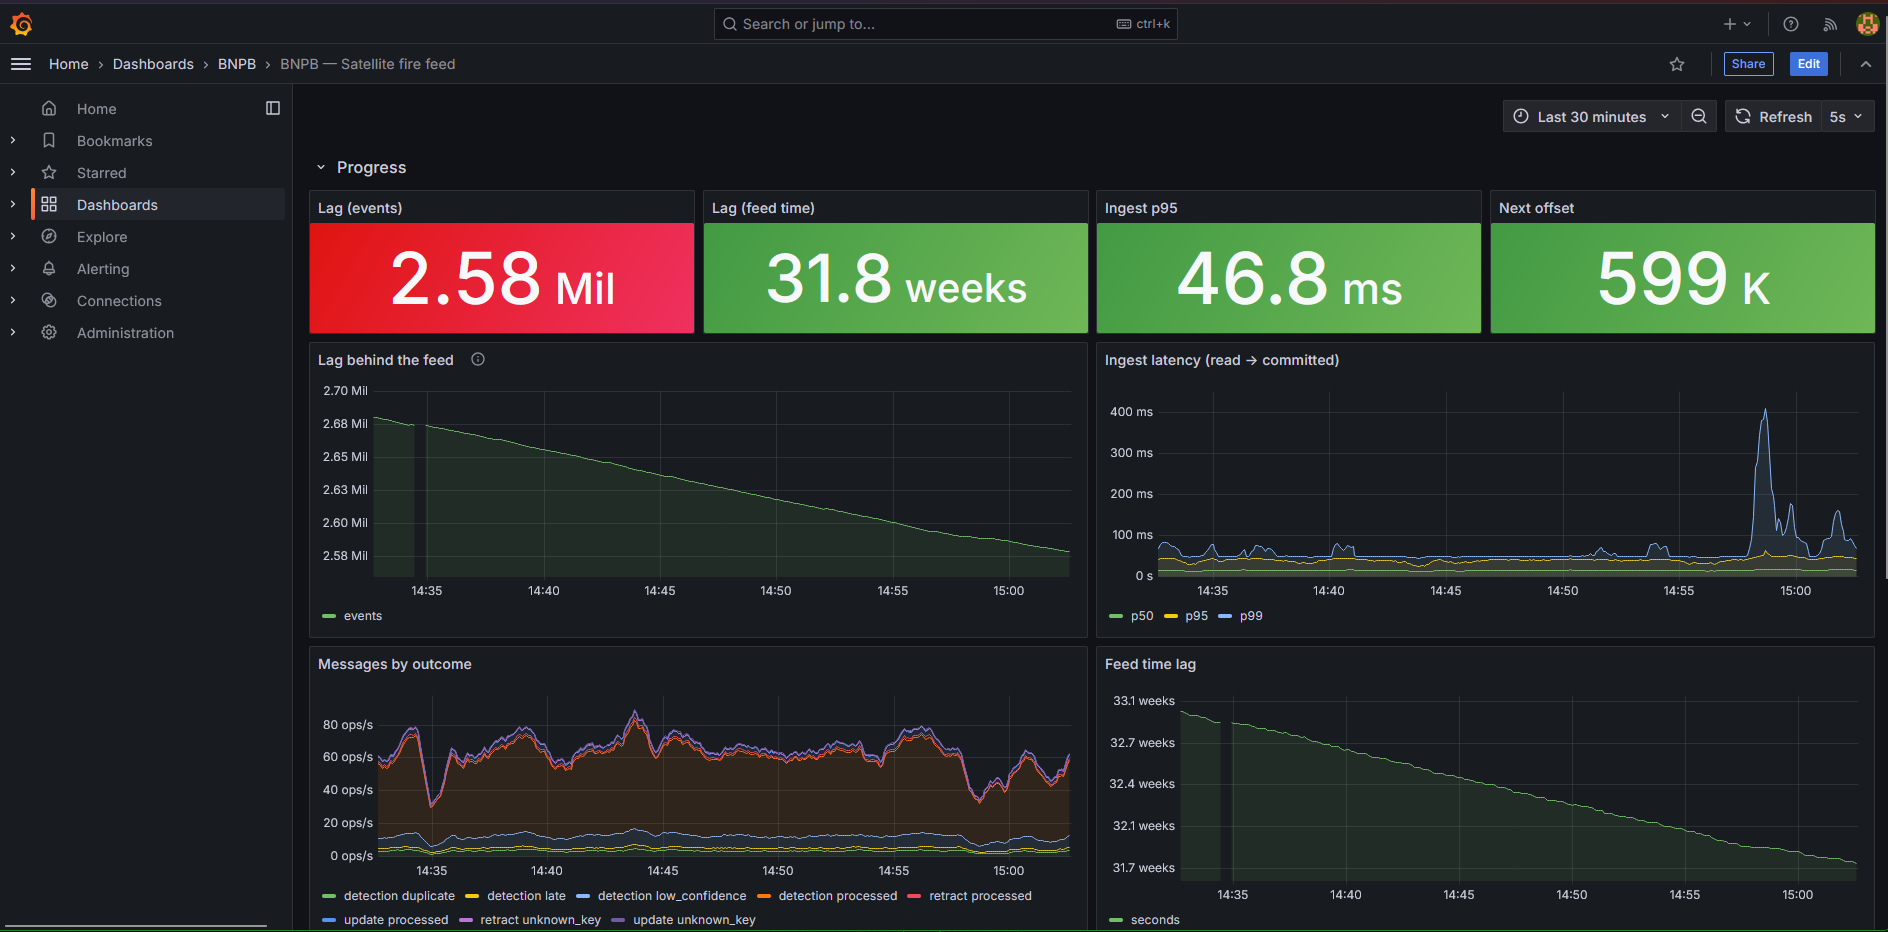
\includegraphics[width=\textwidth]{gambar/satellite-dashboard.png}
\caption{Dashboard \textit{Satellite fire feed} (Docker Compose, 30 menit). Lag $\pm$2,6 juta event berwarna merah karena ambang 1.000 event dibuat untuk keadaan normal. Kurvanya terus turun karena ingestor membaca lebih cepat daripada feed dan menghabiskan sisa \textit{backlog}. Latensi dari baca sampai komit p95 $\pm$47 ms.}
\label{fig:satellite-dashboard}
\end{figure}

\subsubsection{Jawaban atas Butir ``Di Laporan''}
\begin{enumerate}
\item \textbf{Persoalan:} kriteria 2 \textit{event time vs processing time}, \textit{watermark}, \textit{allowed lateness}. Kriteria 4 \textit{consumer lag / backpressure}. Kriteria 5 \textit{stateful processing} dengan \textit{atomic checkpoint} (\textit{exactly-once processing}).
\item \textbf{Pola M1:} \textit{polling} ditinggalkan untuk sumber ini dan diganti konsumsi aliran SSE dengan \textit{offset}. Pola M1 (\textit{polling} berkala dengan \textit{watermark} waktu) cocok untuk API yang hanya bisa ditanya. Feed satelit justru mendorong event berurutan dengan \textit{offset} yang dapat dilanjutkan, sehingga \textit{polling} hanya menambah jeda dan risiko celah. Jalur keluar memakai pola M1 yang sama: \textit{transactional outbox} lalu JetStream, kemudian Aggregator melakukan \textit{upsert} idempoten.
\item \textbf{Kapan kebakaran ``selesai dikenali'', keterlambatan, dan keadaan sementara:} kebakaran tidak ditutup pada jendela tetap. Setiap deteksi baru, \textit{update}, atau \textit{retract} memperbarui kebakaran yang bersangkutan dan dipublikasikan sebagai versi baru. Deteksi yang lebih tua 2 jam dari deteksi terbaru dihitung sebagai \textit{late}. Keadaan (deteksi, kebakaran, \textit{offset}, \textit{outbox}) tersimpan di \kode{satellite-store} dalam satu transaksi. Keadaan sementara terlihat oleh klien sebagai versi kebakaran yang terus bertambah (\kode{source\_version} naik). Klien selalu membaca versi terakhir dan tidak perlu menunggu kebakaran ``selesai''.
\item \textbf{Jaminan pemrosesan:} \textit{exactly-once} secara efektif: \textit{offset} dan keadaan dikomit atomik, \textit{outbox} + \kode{Nats-Msg-Id} + \textit{version guard} di Aggregator mencegah duplikat. Bukti: uji \textit{kill-and-restart} pada kriteria 5.
\end{enumerate}
